\subsubsection{Partitionnement de documents}

Il y a un type d'apprentissage que nous n'avons pas encore abordé, l'apprentissage non supervisé.
Le principe pour le système utilisant ce type d'apprentissage est de tenter de trouver des structures sous-jacentes à partir de données non étiquetées.
Dans notre cas, les données non étiquetées correspondent aux documents bruts, non classés.

Un apprentissage non supervisé doit permettre de mettre en évidence des caractéristiques communes à des données, afin de les organiser par groupes ne contenant que des données similaires.

Dans notre cas, un système de partitionnement des documents pourrait être utile pour organiser automatiquement les documents.
Un avantage est que ces systèmes nécessitent des données qui n'ont pas préalablement été classées.

Les systèmes de partitionnement de documents sont beaucoup utilisés pour les moteurs de recherches.
En effet, il est courant d'obtenir des milliers de pages de résultats pour une requête et le partitionnement des résultats en catégories permet de déterminer ceux qui sont le plus susceptibles d'intéresser l'utilisateur.
Dans notre cas on pourrait par exemple imaginer un système de recherche de documents au sein de la GED qui permette de trier les documents sur les classes générées par le système.
On pourrait même utiliser un système de partitionnement de documents en plus d'un système de classification et ainsi effectuer un partitionnement sur les factures qui permettrait de les regrouper automatiquement par clients, etc.
Le partitionnement de documents pourrait donc s'employer à l'importation de nouveaux documents ainsi que durant les recherches avancées des utilisateurs.
Les utilisations possibles sont multiples.

Afin d'effectuer un partitionnement sur des documents, il est nécessaire de faire certaines préparations préalables.
Au même titre que pour la classification il faut nettoyer le texte de la ponctuation et des <<~mots vides~>>, avant d'appliquer la méthode TF-IDF abordée plus tôt, ou une méthode comparable.
On peut ensuite commencer le processus de partitionnement sur les caractéristiques ainsi extraites.

Des recherches sont en cours dans le domaine du partitionnement afin d'y appliquer des méthodes d'apprentissage profond, mais nous allons ici voir des méthodes plus courantes.
Il existe actuellement quatre catégories d'algorithmes de partitionnement de données.

\paragraph*{Le partitionnement en \textit{k}-moyennes}
~\\

Cette méthode permet de partitionner des données en $k$ groupes, de façon à minimiser la fonction de distance entre les données d'un même groupe.

Pour cette méthode il est nécessaire de choisir à l'avance la valeur de $k$ qui détermine le nombre de groupes.
Lorsque le nombre de groupes voulus est déjà connu, il suffit de renseigner $k$ en conséquence, mais lorsque ce n'est pas le cas il faut appliquer une méthode pour le déterminer.

La méthode généralement appliquée est la <<~elbow method~>>, la méthode du coude.
Elle consiste à tracer une courbe exprimant les valeurs de $k$ testées en fonction de la variance obtenue.
La variance se calcule en divisant la variance entre les groupes par la variance entre toutes les données.
La courbe ainsi obtenue forme un coude et c'est la valeur $k$ en ce point qu'il faut choisir.

Le principal désavantage est que pour déterminer la meilleure valeur de $k$ il faut exécuter l'algorithme pour toutes les valeurs testées.
Un second désavantage est que la méthode définit toujours les groupes avec des tailles similaires, même si cela n'est pas adapté à la situation, comme on peut le voir ci-dessous, le groupe vert devrait être plus important que les bleus et rouges.

\FloatBarrier
\begin{figure}[h!]
    \begin{minipage}[c]{0.45\textwidth}
        \begin{center}
            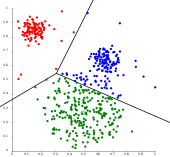
\includegraphics[width = 0.5\textwidth]{k_means}
        \end{center}
    \end{minipage}\hfill
    \begin{minipage}[c]{0.45\textwidth}
        \caption{Partitionnement de données en appliquant la méthode des \textit{k}-moyennes}
        \label{figure:k_means}
    \end{minipage}
\end{figure}
\FloatBarrier

Cette méthode fait partie des méthodes de base qui sont enseignées pour la facilité de leur mise en place, mais les cas d'utilisations en situations réelles sont plutôt rares.

\paragraph*{Le regroupement hiérarchique}
~\\

Les méthodes de regroupement hiérarchique présentent l'avantage de ne pas avoir besoin de déterminer à l'avance le nombre de groupes à créer.
Un autre avantage est qu'elles permettent une visualisation de la hiérarchie créée via un dendrogramme, qui est un type de diagramme.

Le but étant de placer chaque document existant au sein de l'architecture, il y a deux approches possibles~:~par agglomération ou par division.
\\
\begin{itemize}
    \item[\tiny$\bullet$] L'approche par agglomération consiste à initialement considérer chaque document comme un groupe à part entière.
    Ces derniers sont ensuite regroupés par leurs caractéristiques communes les plus proches jusqu'à ne former qu'un seul groupe.
    \item[\tiny$\bullet$] L'approche par division est l'exact opposé, on débute avec un seul groupe englobant la totalité des données.
    Ensuite, on sépare les données en groupes de plus en plus petits en fonction des caractéristiques, jusqu'à ce que tous les documents soient séparés dans des groupes individuels.
\end{itemize}
~\\

Ces méthodes permettent de générer une architecture hiérarchique que l'on peut facilement visualiser.

Ce type de regroupement est fortement efficace sur des données possédant des relations hiérarchiques fortes entre elles.
Les documents stockés au sein d'une GED ne possèdent pas forcément de lien hiérarchique, par conséquent, ce type de regroupement n'est peut-être pas l'idéal pour notre cas de figure.

\paragraph*{Le partitionnement basé sur les lois de probabilités}
~\\

Ce modèle est basé sur des lois de probabilités.
Les groupes sont définis comme des objets appartenant à une même distribution de probabilité.

Ce type de partitionnement diffère des autres de par le fait qu'ici tous les éléments font partie de chaque groupe, mais avec un degré d'appartenance différent.
Par exemple, sur l'image ci-dessous on peut voir que les points bleus font partie du groupe rouge, cependant leur degré d'appartenance au groupe bleu est plus fort.

\FloatBarrier
\begin{figure}[h!]
    \begin{minipage}[c]{0.45\textwidth}
        \begin{center}
            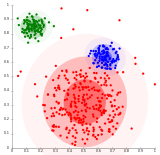
\includegraphics[width = 0.5\textwidth]{distribution}
        \end{center}
    \end{minipage}\hfill
    \begin{minipage}[c]{0.45\textwidth}
        \caption{Visualisation d'un partitionnement effectué en utilisant la loi de probabilité normale}
        \label{figure:distribution}
    \end{minipage}
\end{figure}
\FloatBarrier

Cette méthode est généralement combinée avec la méthode des $k$-moyennes, car il est nécessaire de déterminer préalablement le nombre $k$ de groupes à former.
Cependant, les deux méthodes combinées permettent de donner de très bons résultats.

\paragraph*{Le partitionnement sur la densité}
~\\

L'algorithme le plus populaire de cette catégorie est le DBSCAN (density-based spatial clustering of applications with noise), il se base sur les zones présentant une densité de points supérieure au reste de l'espace des données, pour les regrouper par groupes.

Cet algorithme permet de déterminer par lui-même le nombre de groupes à trouve.
Il est capable de gérer les données aberrantes et ainsi est très peu sensible au bruit.
C'est cette dernière raison qui en fait un algorithme autant utilisé dans le domaine.
En revanche, il ne permet pas une définition précise des bords de chaque groupe, car il est courant que la densité des points soit moins haute à ces endroits.

\paragraph*{Conclusion}
~\\

Aucune méthode de partitionnement de données ne donne de résultats parfaits, mais il est important de noter que les applications de ces méthodes ne nécessitent généralement pas un partitionnement précis.

Selon le cas de figure, il peut être intéressant d'utiliser soit la méthode de partitionnement utilisant les distributions de probabilité, soit celle utilisant la densité.

La première garantie que toutes les données appartiennent à un groupe.
Il peut donc être intéressant de l'utiliser à l'importation d'un nouveau document au sein de la GED afin de garantir qu'il soit classé dans un groupe.

Si l'on souhaite plutôt appliquer une méthode de partitionnement au moment d'une recherche par un utilisateur il peut être intéressant d'utiliser le partitionnement basé sur la densité.
Puisque dans ce cas on souhaite diriger l'utilisateur vers les documents les plus susceptibles de l'intéresser.